\section{Pointer Tagging}
\label{sec:preliminaries:pointertagging}

Pointer Tagging \cite{taggedpointer} is a low-level programming technique that uses the spare low bits in a pointer to encode additional information. Using the Pointer tagging technique, pointer value (initially a memory address before tagging) can hold extra information, \textit{a tag}. The tag can hold extra information about the point-to heap object or can be used as meta-data to further describe the usage of the pointer data. Pointer tagging is mainly enabled because of the way heap objects are situated and accessed on modern computer architectures.

\subsection{Data Structure Alignment}
\label{sec:preliminaries:data_alignment}
Data alignment (also referred to as data structure padding) is a way in which heap objects are arranged and accessed by the CPU. CPUs in modern computer architecture (say 64-bit architecture) read data from and write data to memory more efficiently when data is aligned.  \\

On an abstract level, computer memory can be seen as an array of words or bytes, each with its own address. Unlike bytes, the term word has ambiguate meaning. In the context of this work, we are targeting the generic term in the context of CPU architecture. That is, a "processor word" refers to the size of a processor register or memory address register. The term word also refers to the size of CPU instruction, or the size of a pointer depending on the exact CPU architecture \cite{OSConcept}. For example, in a 64-bit architecture, the word size (also pointer size) is 64 bits = 8 bytes.\\

Generally, when a source program is executed, it is loaded into memory and put into a process $p$ for execution. All data objects in the program are mapped at certain point in time (during compilation or execution) to a physical memory address \cite{OSConcept}. Let us take, as an example, the following coding snippet written in C++:

\begin{verbatim}
bool *p1 = new bool(true);     // p1 = 0x011F0
int  *p2 = new int(123);       // p2 = 0x11608
char *p3 = new char(‘A’);      // p3 = 0x117A8
\end{verbatim}

The execution of the snippet will metaphorically results in a memory layout similar to the one presented in figure \ref{fig:data_aligntment}. According to C++ language specification \cite{cpp}, the size of integer value in memory is 4 bytes, the size of char is 1 byte, and short is 2 bytes. When we execute the previously mentioned statements, however, the compiler (or linker) books 8 bytes of memory to hold the integer value and not 4 bytes as expected. The reason is that, the compiler adds padding to the heap objects in order to align them in memory. The same applies to the character value (Fig. \ref{fig:data_aligntment}).  \\

Why data alignment? The CPU can access the memory only in word-sized chunks. So if our data always starts at a word it can be fetched efficiently. If data was to start somewhere in the middle of a word, the CPU will need to wait two or more memory cycles to fetch data from or write data to memory causing an increase in the CPU \textit{stall} period which results in a significant performance overhead  \cite{OSConcept}. \\


many modern compilers implementations handle data alignment in memory automatically, example includes C, C++, Rust, C\# compilers.

\begin{figure}
	\centering
	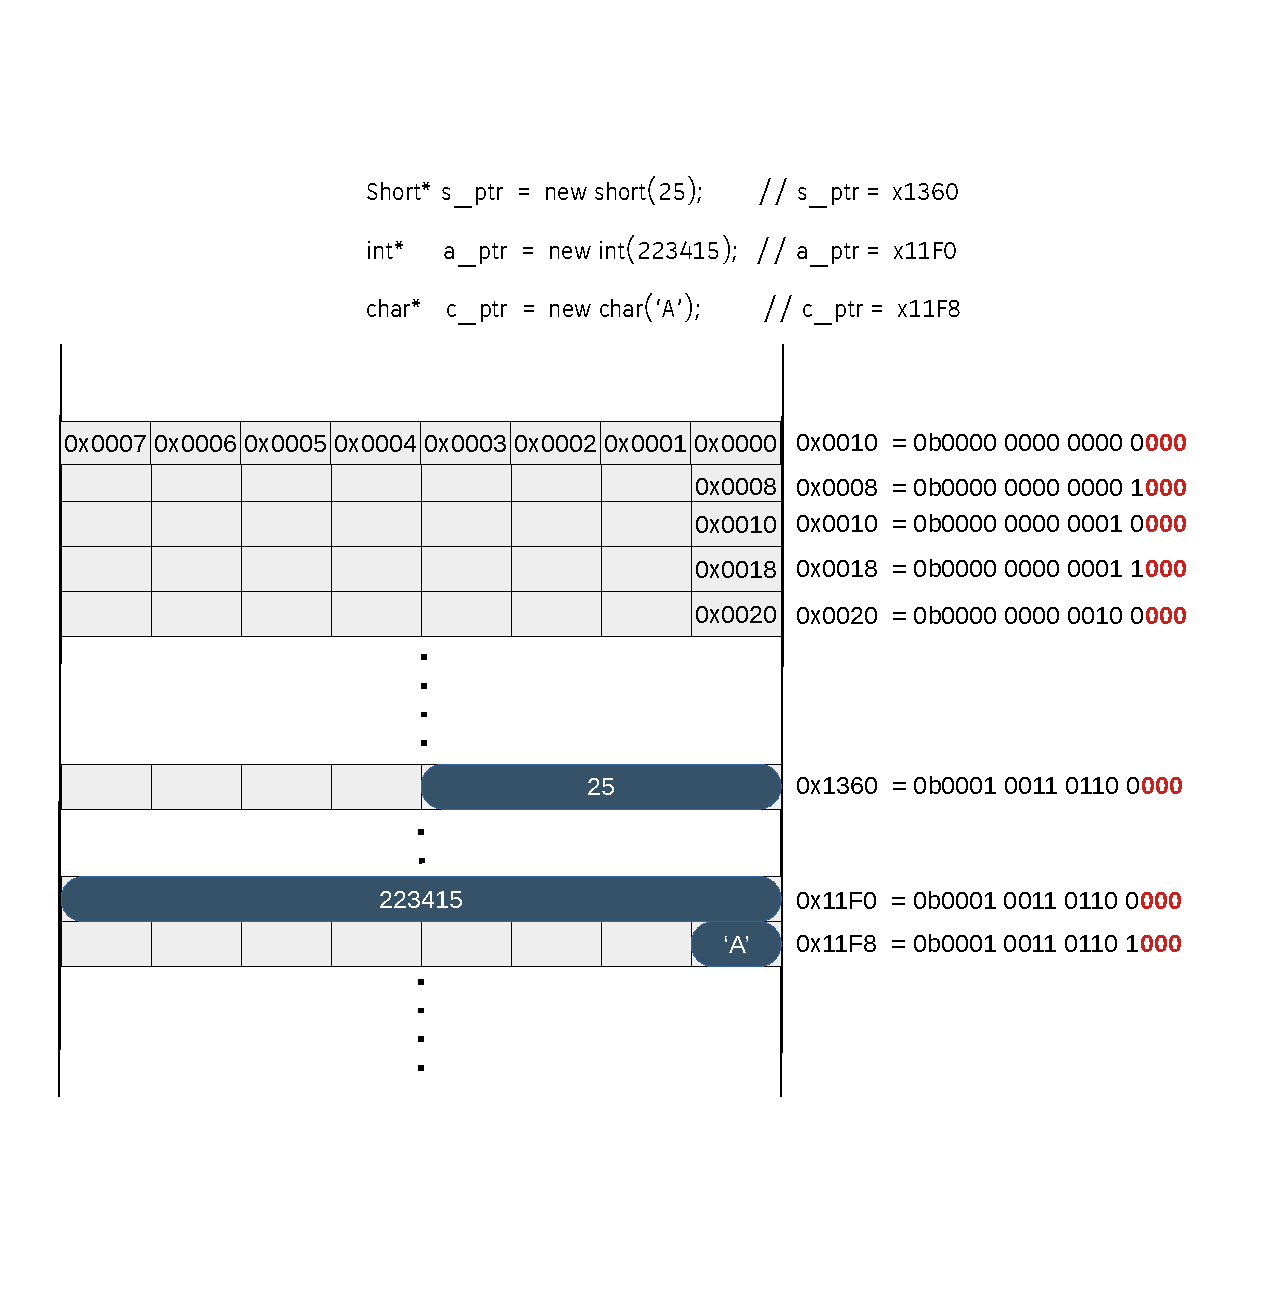
\includegraphics[scale=0.8]{figures/chapter2/memorylayout}
	\caption{An example of memory layout with data objects of various types allocated in the heap. All objects are aligned by 8 bytes so their addresses are always multiple of 8.}
	\label{fig:data_aligntment}
\end{figure}

\subsection{Tagged Pointers}
Some high-level programming languages, for example C++, offer developers a tool set to work with memory. Using such tool set, developers have access to low level memory abstraction. The main building block that enables memory management is the \textbf{pointer data type} and its ecosystem. A variable of type pointer holds a memory address of an object stored in the heap. Due to data alignment (cf. \ref{sec:data_alignment}), the memory address of any object in the heap memory is always $\alpha\cdot w$ where $w=8$ (the word size). This implies all addresses held as a pointer value are multiple of 8. A pointer thus can be 8, 16, 24, 109144, etc. But it can not be 7 or 13. \\

\begin{figure}
	\centering
	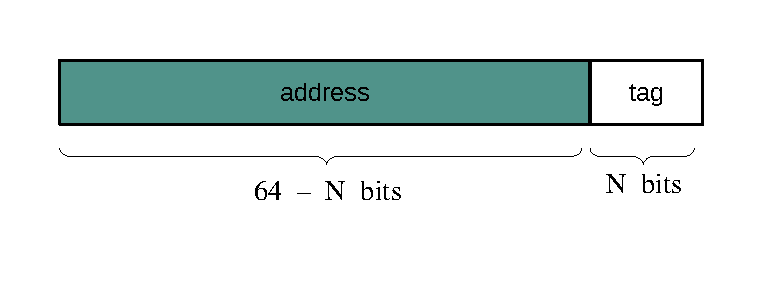
\includegraphics[scale=1]{figures/chapter2/pointervalue}
	\caption{The structure of a tagged pointer. The number of tagging bits depends on the CPU architecture. Depending on the architecture, a $ N = log_{2}(word\_size)$ of LSBs bits are dedicated for tagging. In 64-bit architecture, $word_size = 8$, thus $N = 3$.}
	\label{fig:tagged_pointer}
\end{figure}


Consequently, all pointer values share the fact that the first three low significant bits (LSBs) in their binary representation are always 0. As a result, we could exploit those bits to encode additional information without affecting the validity of the pointer (Fig. \ref{fig:tagged_pointer}).  \\ 

As a use case, depending on the tag, pointer tagging allows a dynamic representation of the numeric value held by the pointer. Thus, the actual payload of the pointer could represents a memory address for some time during the process execution but can later express the binary representation of a \texttt{char} value for example, depending on the execution context and after a change in the tag value during run-time. \\

\subsection{Tagged Pointer Implementation}

An approach to implement a tagged pointer is to develop a wrapper object around a pointer type variable. By that, we insure safety by presenting a single point of failure in case of pointer value misuse. The wrapper can be equipped with adequate behaviours that govern the tag/ payload manipulation and retrieval. \\

Accessing the binary representation of pointer to enable pointer tagging is straightforward in most programming languages and is done by using bit-wise operations. \\


\clearpage